\documentclass{beamer}

%%%%%%%%%%%%%Solarized Theme%%%%%%%%%%%%%%%
\usecolortheme[dark,accent=cyan]{solarized}
\beamertemplatenavigationsymbolsempty
%%%%%Packages%%%%%
\usefonttheme{serif}
\usepackage[T1]{fontenc}
\usepackage[utf8]{inputenc}
\usepackage[english]{babel}
\usepackage{fontawesome}
\usepackage{minted}
\usepackage{soul}
\usepackage{ulem}
\usepackage{blkarray}
\usepackage{multirow}

\definecolor{DarkGray}{gray}{0.1}
\usemintedstyle{paraiso-dark}


\usepackage{graphicx}
\usepackage{hyperref}
\usepackage{colortbl, xcolor}
\usepackage{booktabs}
\usepackage{amsmath,amsthm, amssymb, latexsym}

\usepackage{tikz}
\usepackage{xcolor}
\usepackage{graphicx,multirow}
\definecolor{plain}{rgb}{93,93,93}
\usetikzlibrary{positioning,arrows}
\definecolor{applegreen}{rgb}{0.55, 0.71, 0.0}
\usetikzlibrary{decorations.pathreplacing, backgrounds, fit}
\usetikzlibrary{calc,matrix}

\tikzstyle{background}=[solarizedRed, rectangle, draw, inner sep=1mm, thick,
           rounded corners=2mm]

\tikzset{
  treenode/.style = {align=center, inner sep=0pt, text centered,
    font=\sffamily},
  arn_n/.style = {treenode, circle, white, font=\sffamily\bfseries, draw=black, inner sep=-6pt,
    fill=black, text width=1.5em},% arbre rouge noir, noeud noir
  arn_r/.style = {treenode, circle, red, 
    text width=1.5em, very thick, inner sep=4pt},% arbre rouge noir, noeud rouge
  arn_x/.style = {treenode, rectangle, draw=black,
    minimum width=0.5em, minimum height=0.5em}% arbre rouge noir, nil
}

\usepackage{standalone}
\usepackage{siunitx}

\begin{document}

\begin{frame}
    \begin{center}
        \Large{\textcolor{orange}{Saving Face: Investigating the Ethical Concerns of Facial Recognition Auditing}} \\
    
        \vspace{1cm}
        \normalsize{@NikoletaGlyn} \\
        \vspace{.5cm}
        
\includegraphics[width=0.14\textwidth]{static/dyno.png}

    \end{center}
\end{frame}

\begin{frame}
    \centering
    \footnotesize{
    \begin{minipage}[t]{0.3\textwidth}
        \centering
        Inioluwa Deborah Raji \\
        University of Toronto
    \end{minipage}
    \begin{minipage}[t]{0.3\textwidth}
        \centering
        Timnit Gebru \\
        Google Research
    \end{minipage}
    \begin{minipage}[t]{0.3\textwidth}
        \centering
        Margaret Mitchell \\
        Google Research
    \end{minipage}}
    \vfill

    \footnotesize{
    \begin{minipage}[t]{0.3\textwidth}
        \centering
        Joy Buolamwini \\
        MIT Media Lab.
    \end{minipage}
    \begin{minipage}[t]{0.3\textwidth}
        \centering
        Joonseok Lee \\
        Google Research
    \end{minipage}
    \begin{minipage}[t]{0.3\textwidth}
        \centering
        Emily Denton \\
        Google Research
    \end{minipage}}
\end{frame}

\begin{frame}
    \centering
    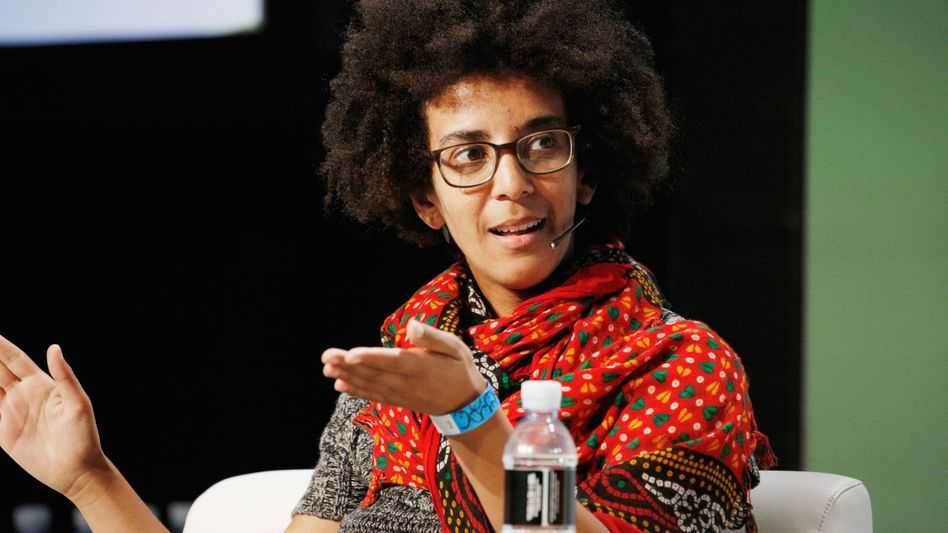
\includegraphics[width=.75\textwidth]{static/timnit_gebru}
\end{frame}

\begin{frame}
    \centering
    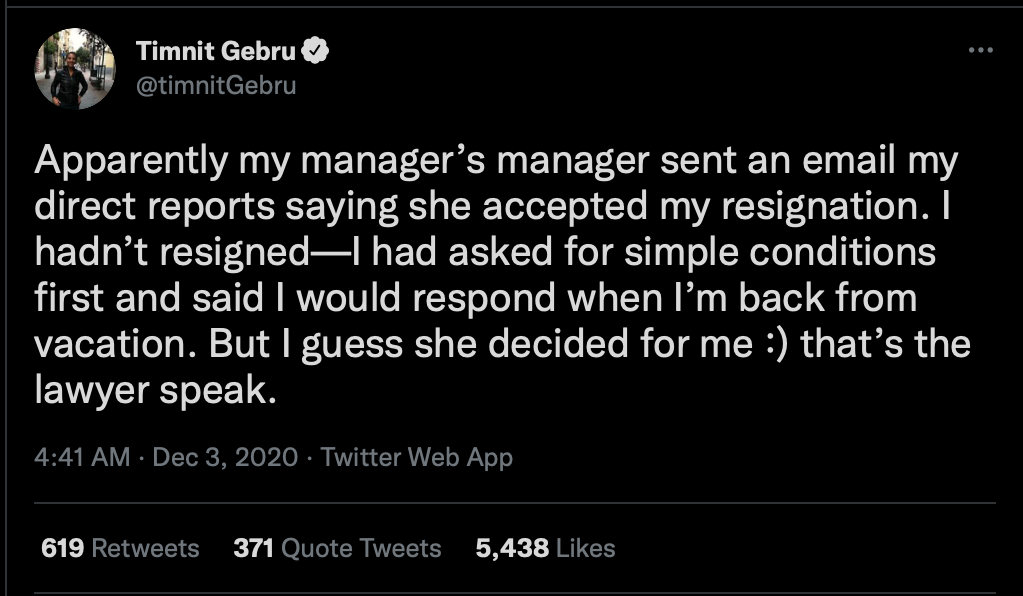
\includegraphics[width=.75\textwidth]{static/timnit_gebru_tweet}
\end{frame}

\begin{frame}
    \centering
    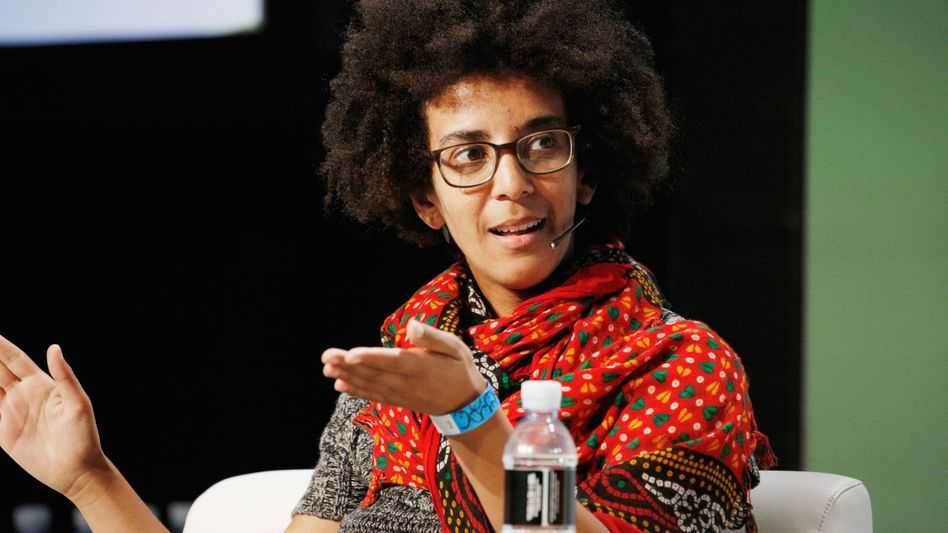
\includegraphics[width=.75\textwidth]{static/timnit_gebru}
\end{frame}

\begin{frame}
    \begin{center}
    \LARGE{FACIAL PROCESSING TECHOLOGY}

    % \begin{minipage}{.3\textwidth}
    %     \normalsize{[ko - rektnas]}
    % \end{minipage}
    \vspace{.5cm}

    \hspace{-8cm}\\
    \end{center}
    \normalsize{a broad term that encompasses a variety of tasks ranging from face detection, facial analysis, and face verification or identification.}

\end{frame}

\begin{frame}
    \begin{center}
    \LARGE{CelebSET}
    \end{center}
\end{frame}

\begin{frame}
    \begin{center}
    \LARGE{80 Celebrities} \\
    \LARGE{20 for each group} \\
    \LARGE{LM} \hspace{.5cm} \LARGE{DM} \hspace{.5cm} \LARGE{LF} \hspace{.5cm} \LARGE{DF} \\
    \end{center}
\end{frame}

\begin{frame}
    \begin{center}
        \begin{tabular}{ c | c | c | c | c |c}
         Photo & Ethnicity & Colour & Gender & Age & Smile \\ \midrule
               &           & 1 - 6  & F/M    &  Photo Taken & Y/N
        \end{tabular}
        \end{center}
\end{frame}

\begin{frame}
    \centering
    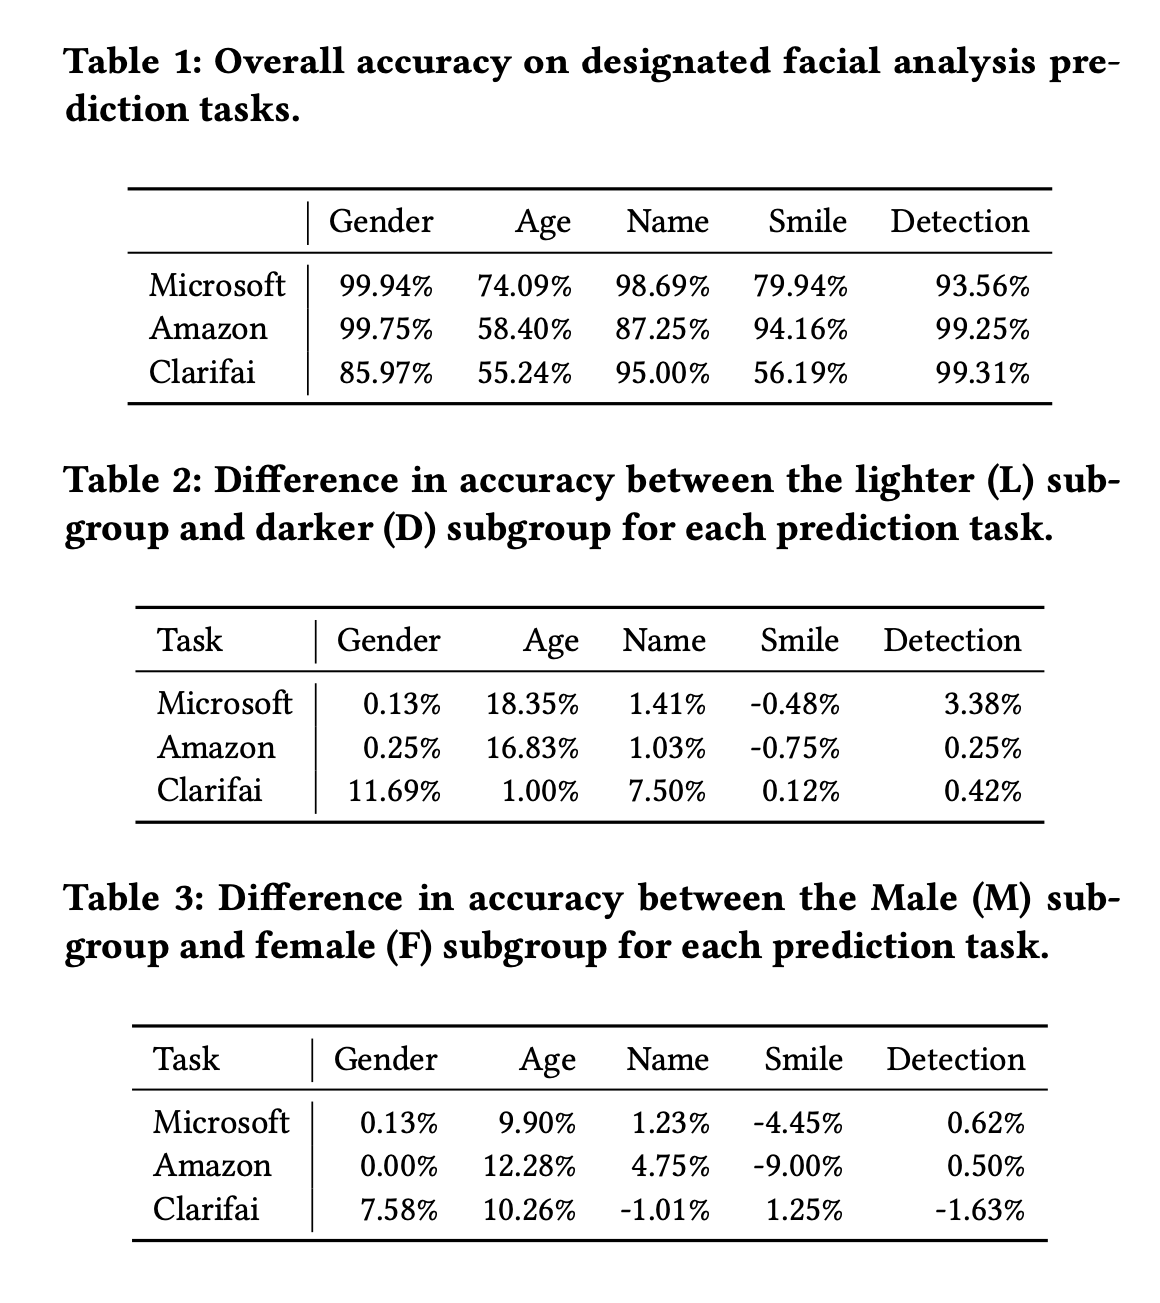
\includegraphics[width=.60\textwidth]{static/results.png}
\end{frame}

\begin{frame}
    \centering
    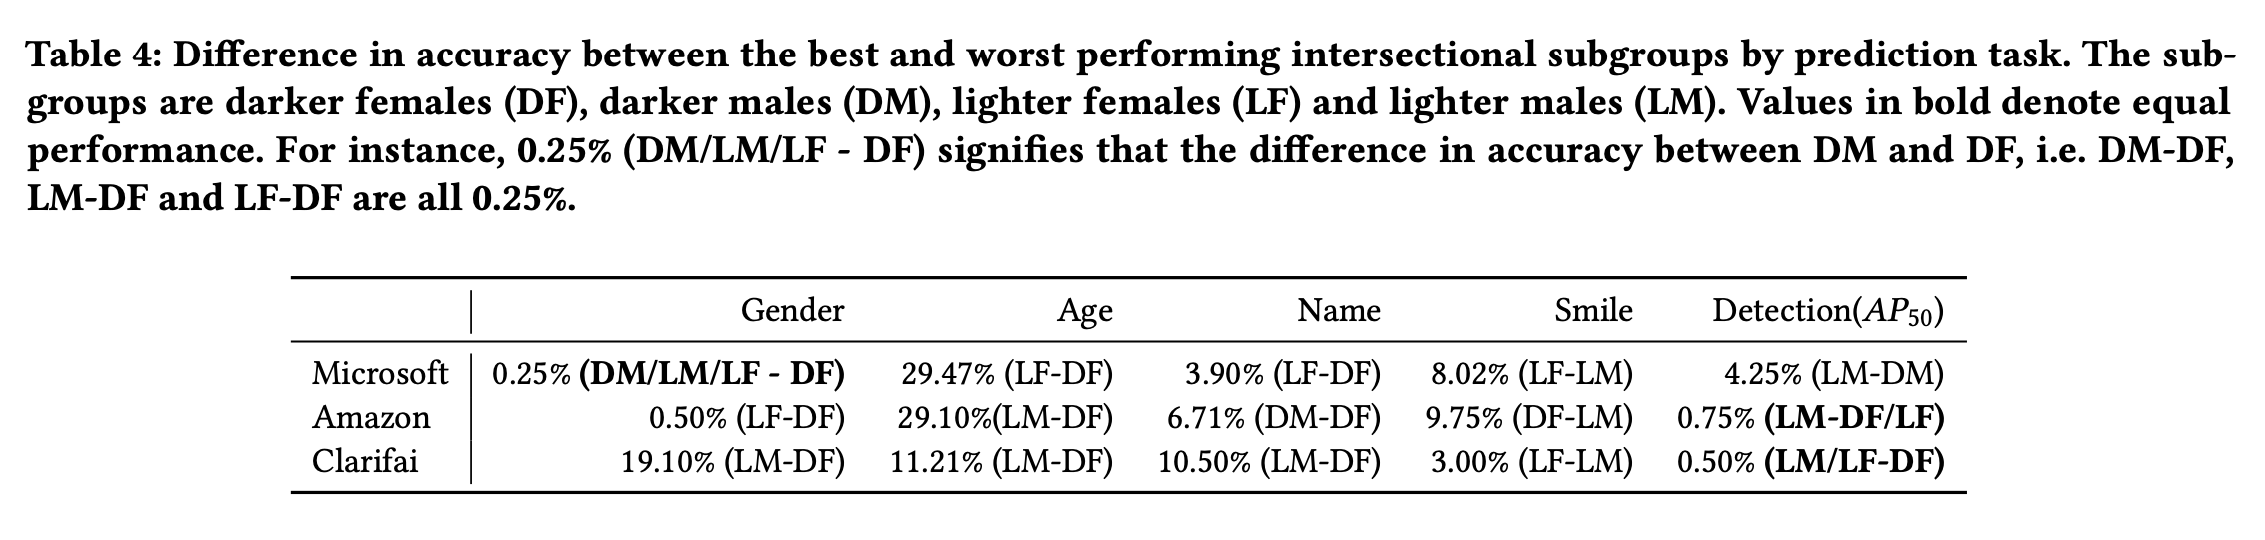
\includegraphics[width=\textwidth]{static/results_two.png}
\end{frame}

\begin{frame}
    \begin{center}
    \LARGE{Design Considerations}
    \end{center}
\end{frame}

\begin{frame}
    \begin{center}
    \LARGE{Consideration 1: Selecting Scope of Impact.}
    \end{center}
\end{frame}

\begin{frame}
    \begin{center}
    \LARGE{Consideration 2: Auditing for Procedural Fairness. }
    \end{center}
\end{frame}

\begin{frame}
    \centering
    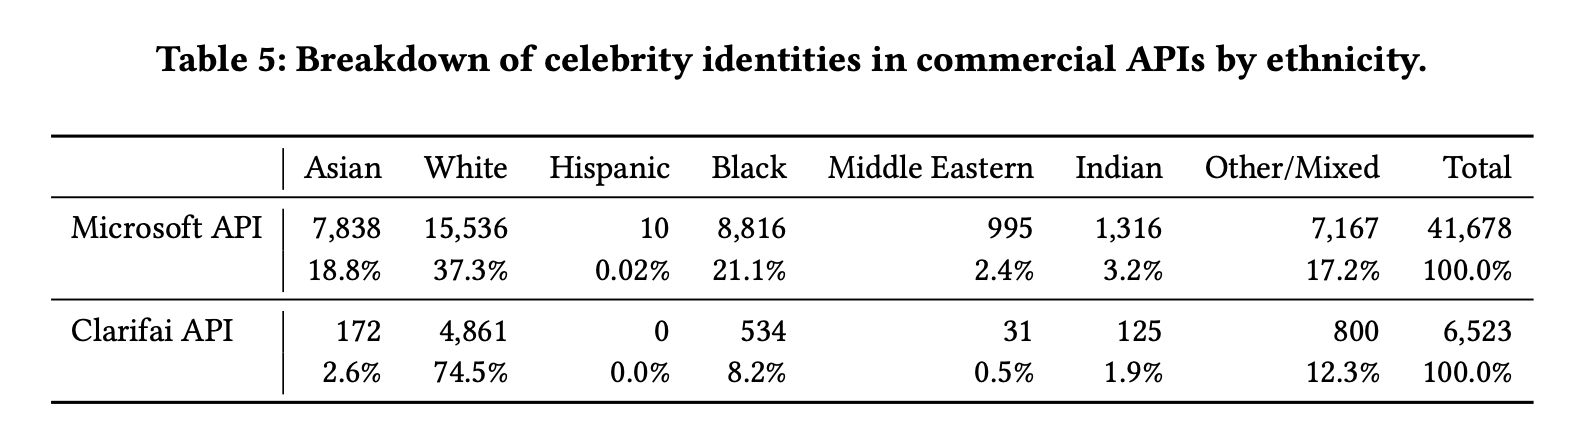
\includegraphics[width=\textwidth]{static/table_five.png}
\end{frame}

\begin{frame}
    \begin{center}
    \LARGE{Ethical Tensions}
    \end{center}
\end{frame}

\begin{frame}
    \begin{center}
    \LARGE{Tension 1: Privacy and Representation.}
    \end{center}
\end{frame}

\begin{frame}
    \centering
    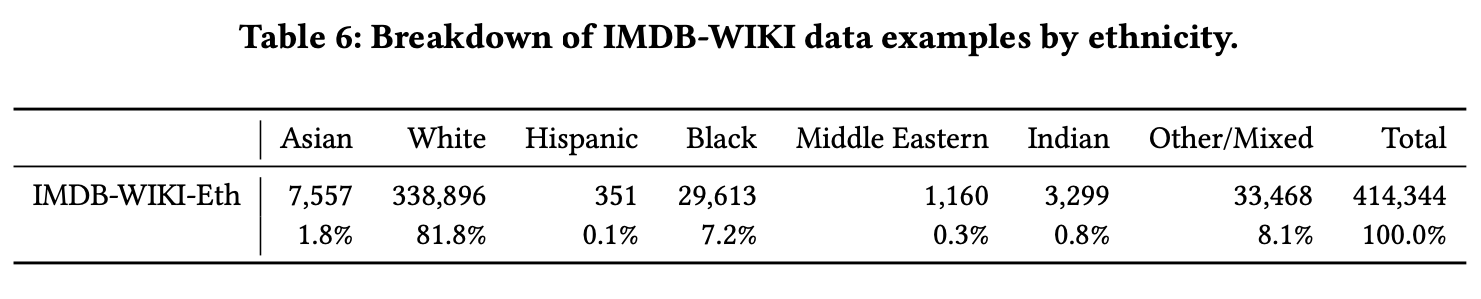
\includegraphics[width=\textwidth]{static/table_six.png} \\ \vfill
    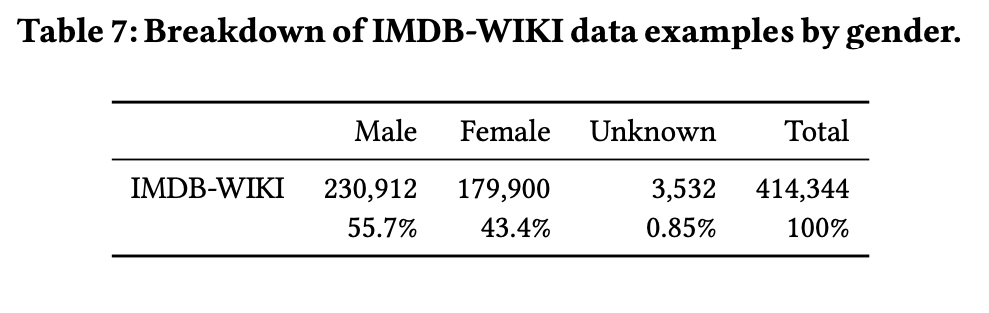
\includegraphics[width=.65\textwidth]{static/table_seven.png}
\end{frame}

\begin{frame}
    \begin{center}
    \LARGE{Tension 2: Intersectionality and Group-Based Fairness.}
    \end{center}
\end{frame}

\begin{frame}
    \begin{center}
    \LARGE{Tension 3: Transparency and Overexposure.}
    \end{center}
\end{frame}

\begin{frame}
	\begin{center}
    \faTwitter \\
    @rajiinio \\
    @timnitGebru \\
    @jovialjoy \\
    @mmitchell\_ai \\
    @cephaloponderer \\
	\end{center}
\end{frame}



\end{document}